\chapter{Aplikácie}

Rozšírená realita má množstvo využití od zábavy až po záchranu životov. Nižšie sú vybrané niektoré z nich.

\section{Medicínske aplikácie}

Rozšírená realita by mohla mať bohaté využitie na poli medicíny. Lekárom by sa pomocou nej mohli vytvárať detailné vizualizácie vnútorných orgánov, nádorov a podobne a zobrazovať sa im prekryte priamo cez telo pacienta. Na získanie údajov by sa mohlo použiť ľubovoľné diagnostické zariadenie, ktoré produkuje 3D dáta o pacientovi. Napríklad vyšetrenie magnetickou rezonanciou, alebo ultrazvukom. Tieto vizualizácie by mohli byť obzvlášť cenné pri minimálne invazívnych zákrokoch, kedy vidí chirurg vnútro tela pacienta horšie, ako pri bežnej operácii \cite{Azuma97}.

Vedci z Mníchovského Institut für Informatik vyvinuli trenažér pre gynekológov na~nácvik pôrodov, ktorý využíva rozšírenú realitu. Pôvodný simulátor, ktorý vypisoval fiziologické dáta ako sú krvný tlak, tep, úroveň bolesti, či údaje o prívode kyslíka na monitor pristavený pri nemocničnej posteli, prestavali tak, aby sa všetky potrebné údaje vypisovali na okuliare špeciálnej helmy. Okrem vypisovania týchto jednoduchých dát sa však na okuliare dokresluje aj polopriehľadný virtuálny model dieťaťa uloženého v maternici. Na to, aby to bolo možné je potrebné registrovať vzájomnú polohu hlavy používateľa a simulátoru.


Podľa autorov hrá toto dôležitú rolu pri zvyšovaní efektivity tréningu, nakoľko sa lekár môže plne koncentrovať na simulovaný vaginálny pôrod namiesto sledovania počítačových monitorov \cite{Sielhorst04}.

V roku 2004 bol v Kalifornii vykonaný prvý úspešný chirurgický zákrok prevedený za asistencie rozšírenej reality. Štyridsaťpäťročný pacient podstúpil laparoskopickú adrenalektómiu (odobranie nadobličky). Chirurgovi sa pri operácií na monitor zobrazovala 3D rekonštrukcia nadobličiek a iných okolitých orgánov vsadená na správne miesto do pohľadu z kamery. Toto pozíciovanie sa vypočítavalo na základe siedmich markerov nalepených na koži pacienta \cite{Marescaux04}.

\section{Požiarnici}

Patrick Jackson, požiarnik zo Severnej Karolíny vyvíja požiarnicku aplikáciu pre Google Glass. Do okuliarov sa mu premietajú údaje od operátora tiesňovej linky, mapy a ukazovateľ k najbližšiemu hydrantu. V budúcnosti má zobrazovať napríklad aj plány budov, alebo schémy rozrezávania vrakov
jednotlivých modelov áut \cite{Google14-a}. Na zobrazovanie mapy okolia sa využívajú údaje z GPS a na navigovanie k hydrantu aj presné natočenie hlavy. Táto aplikácia je ukážkovým príkladom, ako by mohla rozšírená realita v kritických situáciach zachraňovať životy.

Podobný softvér (s vlastným hardvérom) vyvíja tím na Technickej univerzite vo~Viedni. Požiarnikovi ukazujú v okuliaroch obraz z termálnej kamery registrovaný s~3D modelom štruktúry budovy, ktorý je rekonštruovaný v reálnom čase (obrázok \ref{poziarnici}). Vďaka tomu vie ako vyzerá jeho okolie aj v prípade hustého dymu \cite{Schonauer13}.

\begin{figure}[h]
 \centering
 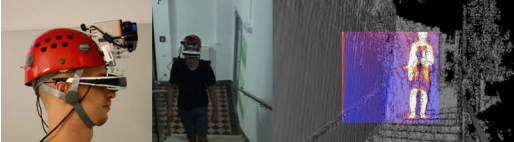
\includegraphics[max width=\textwidth]{pictures/wien-firefighters.png}
 \caption{Projekt má požiarnikom zabezpečiť životne dôležité informácie v podmienkach slabej viditeľnosti \cite{Schonauer13}}
 \label{poziarnici}
 \end{figure}

\section{Preklady}

Na University of California vytvorili mobilnú aplikáciu, ktorá cez rozšírenú realitu prekladá text. Používateľ jednoducho namieri telefón na nápis, ktorý chce preložiť, a~aplikácia text v obraze z kamery zdeteguje pomocou optického rozoznávania znakov. Softvér vzápätí text preloží a vykreslí na obrazovku telefónu priamo do videa z kamery. Pri tomto vložení dbá nielen na to, aby preložený text umiestnil na správne miesto a~v~správnej farbe a veľkosti, ale aj aby vyretušoval pôvodný text, ktorý by bol umiestnený pod tým preloženým \cite{Fragoso11}. Ukážka aplikácie je na obrázku \ref{translatar}.

\begin{figure}[h]
 \centering
 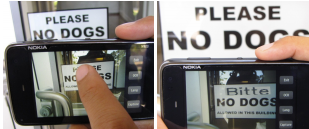
\includegraphics[max width=\textwidth]{pictures/translatar.png}
 \caption{Ukážka aplikácie TranslatAR \cite{Fragoso11}}
 \label{translatar}
 \end{figure}

\section{Armádne aplikácie}

Vojenské operácie sa často vykonávajú v mestskom prostredí. Bojové zóny, v ktorých sa nachádzajú poschodové budovy sú veľmi komplikované a pre~úspech misie sú pre vojaka mimoriadne dôležité informácie o okolí. Keď vojak pozerá do mapy, ohrozuje sa, pretože dáva nižší pozor na svoje okolie.

Vedci z Naval Research Laboratory v USA vytvárajú helmu, ktorá bude vojakom sprostredkovávať najdôležitejšie informácie. Používateľ môže vidieť nad budovami napísané ich mená a plány interiérov, na zemi zas môže vidieť napísané názvy ulíc. Taktiež sa mu môžu zobrazovať ikony na presných lokáciach, kde boli nahlásení ostreľovači~\cite{Livingston02, Julier00}.

Inou aplikáciou rozšírenej reality na armádne účely je systém rozširujúci videnie pilota lietadla. Úlohy ako zameriavanie cieľa, dodávky zbraní a zásob na padákoch, či obyčajný let v nízkej výške vyžadujú, aby pilot presne rozoznával terén pod sebou. Senzory na stíhačke môžu sledovať oblasť, ktorú pilotovi v zornom poli zakrýva samotné lietadlo, alebo mu poskytovať dáta za podmienok slabej viditeľnosti. Všetky tieto dáta sa potom môžu premietať do pilotovej helmy, umožniť mu vidieť to, čo by inak nevidel a zvýrazniť dôležité body \cite{Livingston11}.

Prvé podobné primitívne systémy vznikli už pred Druhou svetovou vojnou. Spojeneckí piloti používali v niektorých lietadlách napríklad Mark II Gyro Sight, teda gyroskopický zameriavač. Toto zariadenie pilotovi ukazovalo na polopriehľadný displej, kam poletí strela na základe údajov z gyroskopu a meraču rýchlosti.

Rozšírená realita prenikla na poli letectva aj do civilnej sféry. Na obrázku \ref{boeing} je pilotná kabína Boeingu pri navádzaní na pristátie.
 
Podobné aplikácie by mohli mať význam aj pre vojenské a civilné pozemné dopravné prostriedky.

\begin{figure}[h]
 \centering
 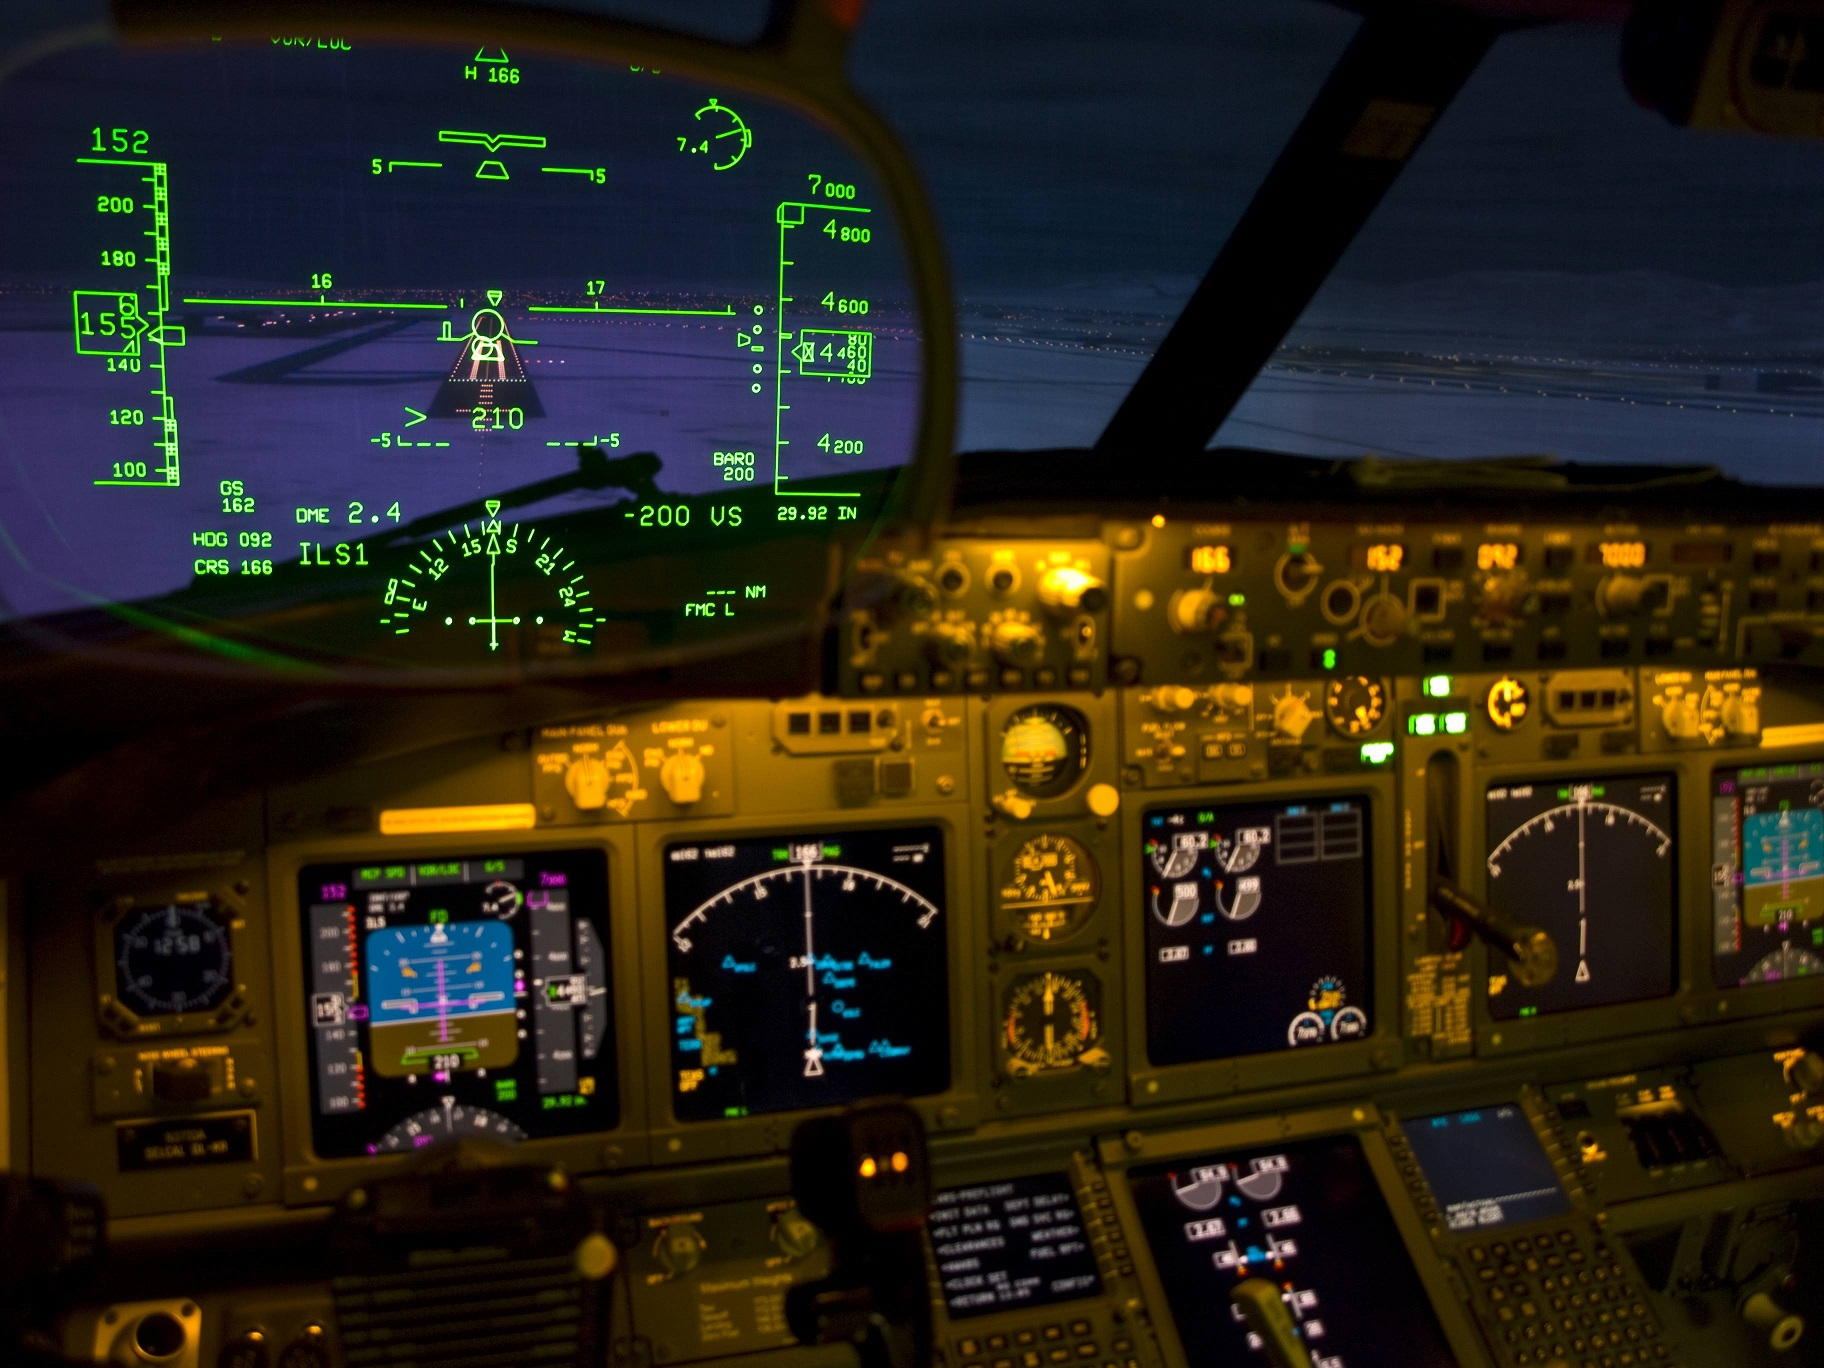
\includegraphics[max width=\textwidth]{pictures/kokpit.jpg}
 \caption{Rozšírená realita v kokpite lietadla Boeing 737-800; Autor: Barend Havenga \cite{Havenga}}
 \label{boeing}
\end{figure}

\section{Šport}

Pri športových televíznych prenosoch je používanie rozšírenej reality pomerne bežné. Prvý krát bol prenos rozšírený už počas Olympijských hier 1996 a napríklad firma Sportvision dodnes virtuálne rozširuje prenášané záznamy už od roku 1998.

Na hraciu plochu dokážu zobrazovať rôzne dočasné čiary a zóny, informácie o bodovom stave, logá, zástavy a podobne a to tak, že sú prekrývané skutočnými hráčmi, ktorí sú na nej. Podobnými spôsobmi rozširujú napríklad televízne prenosy z NHL, NFL, alebo NASCAR \cite{Sportvision, Ismert12}. Mimo Spojených štátov sú zrejme najznámejšími virtuálne zástavy dokreslované do plaveckých bazénov na Olympijských hrách, prípadne čiara, ktorá sa počas preteku posúva pozdĺž bazénu a označuje svetový, alebo Olympijský rekord.

\section{Konštrukcia}

Rozšírená realita by mohla pomôcť aj stavbárom, či statikom. V okuliaroch by im do~reálneho pohľadu mohli byť dokresľované napríklad stĺpy za stenami, presné polohy roxorových tyčí získané magnetickými senzormi, káble vedúce elektrinu v stenách, či~samotné označenia nosných stien \cite{Webster96}.

Iné využitie uľahčuje prácu mechanikom. Napríklad bola vyvinutá aplikácia, ktorá zobrazuje automechanikovi do helmy všetky súčiastky vo dverách auta. Výmena zámku, či motorčeku na otváranie okna je pri tomto modeli vozidla pomerne obtiažna, pretože automechanik musí strčiť ruky dnu do dverí a nevidí, čo robí. Do aplikácie boli nahrané modely všetkých súčiastok a tá ich premieta na
ich skutočné miesto \cite{Reiners98}.